\documentclass[runningheads,a4paper]{llncs}
\usepackage{amssymb}
\setcounter{tocdepth}{3}
\usepackage{listings}
\usepackage{booktabs}
\usepackage{mathtools}
\usepackage{tabularx}
\usepackage{fixltx2e}
\usepackage[hyphens]{url}
\usepackage{hyperref}
\usepackage{upquote,textcomp}
\lstset{breaklines=true, basicstyle=\scriptsize\ttfamily, upquote=true}

\usepackage{fancyvrb}
\VerbatimFootnotes

\usepackage{graphicx}
\makeatletter
\def\maxwidth#1{\ifdim\Gin@nat@width>#1 #1\else\Gin@nat@width\fi}
\makeatother

\usepackage{amsmath}
\usepackage{color,graphics,array,csscolor}
\usepackage{pmml-new}

\usepackage{fontspec,unicode-math}
\usepackage[Latin,Greek]{ucharclasses}
\setTransitionsForGreek{\fontspec{Times New Roman}}{}

\usepackage{subscript}
\lstset{breaklines=true, basicstyle=\scriptsize\ttfamily}

\begin{document}
\mainmatter

\title{The RASH Framework: enabling HTML+RDF submissions in scholarly venues}
\titlerunning{The RASH Framework}
\author{Angelo Di Iorio\inst{1} \and
Andrea Giovanni Nuzzolese\inst{1,2} \and
Francesco Osborne\inst{3} \and \\
Silvio Peroni\inst{1,2} \and
Francesco Poggi\inst{1} \and
Michael Smith\inst{4,5} \and
Fabio Vitali\inst{1} \and \\
Jun Zhao\inst{6}}
\authorrunning{Angelo Di Iorio et al.}
\institute{Department of Computer Science and Engineering, University of Bologna, \\Bologna, Italy\and
Semantic Technology Laboratory, Institute of Cognitive Sciences and Technologies, Italian National Research Council, Rome, Italy\and
Knowledge Media Institute, The Open University, Milton Keynes, United Kingdom\and
World Wide Web Consortium, Shinjuku, Tokyo, Japan\and
Graduate School of Media and Governance, Keio University, \\Fujisawa, Kanagawa, Japan\and
School of Computing and Communications, Lancaster University, \\Lancaster, United Kingdom\\
\email{angelo.diiorio@unibo.it, 
andrea.nuzzolese@istc.cnr.it, 
francesco.osborne@open.ac.uk, 
silvio.peroni@unibo.it, 
francesco.poggi@unibo.it, 
mike@w3.org, 
fabio.vitali@unibo.it, 
j.zhao5@lancaster.ac.uk}}
\maketitle

\begin{abstract}
This paper introduces the {\em RASH Framework}, i.e., a set of specifications and tools for writing academic articles in {\em RASH}, a simplified version of HTML. RASH focuses strictly on writing the content of the paper leaving all the issues about its validation, visualisation, conversion, and data extraction to the tools developed within the framework.

\keywords{Digital Publishing, RASH, Semantic Publishing, Semantic Web, XSLT, document conversion}
\end{abstract}


\section{Introduction}\label{sec_introduction}

In the last months of 2014, several posts within technical mailing lists of the Web and Semantic Web community have discussed an evergreen topic in scholarly communication, i.e., how authors of research papers could submit their works in HTML rather than, say, PDF, MS Word or LaTeX. Besides the obvious justification of simplification and unification of data formats for drafting, submission and publication, an additional underlying rationale is that the adoption of HTML in the context of scientific publications would ease the embedding of semantic annotations, thus making a step towards the improvement of research communications thanks to already existing W3C standards such as RDFa and Turtle. The adoption of Web-first formats in scientific literature, i.e., HTML and RDF, is a necessary step towards the complex (and exciting) scenarios that the Semantic Publishing has promised us  \cite{force11} \cite{shotton-sempub}. However, such formats should support the needs of the actors involved in the production/delivery/use of scholarly articles.

Along the lines of other existing works on this topic (e.g., {\em Linked Research} project  \cite{linked-research} and {\em ScholarlyMarkdown} \cite{scholmd}), in this paper we introduce the {\em RASH Framework}, i.e., a set of specifications and tools for writing academic articles in {\em RASH} (an HTML+RDF-based markup language for writing scholarly documents) which aims at addressing all the aforementioned issues.

The rest of the paper is structured as follows. In Section~\ref{sec_rationale} we introduce the rationale for the RASH Framework. In Section~\ref{sec_tools} we provide a quick overview of all its tools, that are available in the Framework repository. Finally, in Section~\ref{sec_conclusions} we conclude the paper sketching out some future developments.

\section{A ``Web-first'' framework for research articles}\label{sec_rationale}

Some works, e.g., Capadisli {\em et al.} \cite{linked-research}, suggest not to force any particular HTML structure for research papers. In this way, the author of a paper is free to use any possible kinds of HTML {\em linearisations} for writing a scholarly text. This freedom could, however, results in two main kinds of issues:
\begin{itemize}
\item {\em visualisation bottleneck} -- it may affect the correct use of existing, well-developed and pretty standard CSSs;
\item {\em less focus on the research content} -- the fact that a certain paper is not visualised in a browser very well could bring the author to work on the presentation of the text, rather than on its research content.
\end{itemize}

A further complication to an already complex scenario comes from the {\em necessary} involvement of publishers. Leaving the authors free of using their own HTML format could be also counterproductive from a publisher's perspective, in particular when we speaking about the possibility of adopting such HTML formats for regular conference/journal camera-ready submissions.

The RASH Framework\footnote{The full project is available at \url{https://github.com/essepuntato/rash/}. Please use the hashtag \verb+#rashfwk+ for referring to any of the items defined in the RASH Framework via Twitter or other social platforms.} has been proposed in order to address all the aforementioned issues. It is a set of specifications and tools for writing academic articles in {\em RASH} - a summary of the whole framework is introduced in Fig.~\ref{fig_framework}.

The {\em Research Articles in Simplified HTML} ({\em RASH}) format is a markup language that restricts the use of HTML elements to only {\em 25 elements} for writing academic research articles, and it is entirely based on a strong theory on {\em structural patterns} for XML documents  \cite{patterns}. It allows authors to use RDFa annotations within any element of the language. In addition, RASH allows the use of elements \verb+script+ (with the attribute \verb+type+ set to ``text/turtle'' or to ``application/ld+json'') within the element \verb+head+ for adding plain Turtle or JSON-LD content. Any RASH documents begins as a simple (X)HTML5 document\footnote{Please refer to the official RASH documentation, available at \url{http://cs.unibo.it/save-sd/rash}, for a complete introduction of all the elements and attributes that can be used in RASH documents.}, by specifying the document element \verb+html+ (with the usual namespace) that contains the element \verb+head+ for defining metadata of the document, and the element \verb+body+ for including the whole content of the document.
\begin{figure}[h!]
\centering
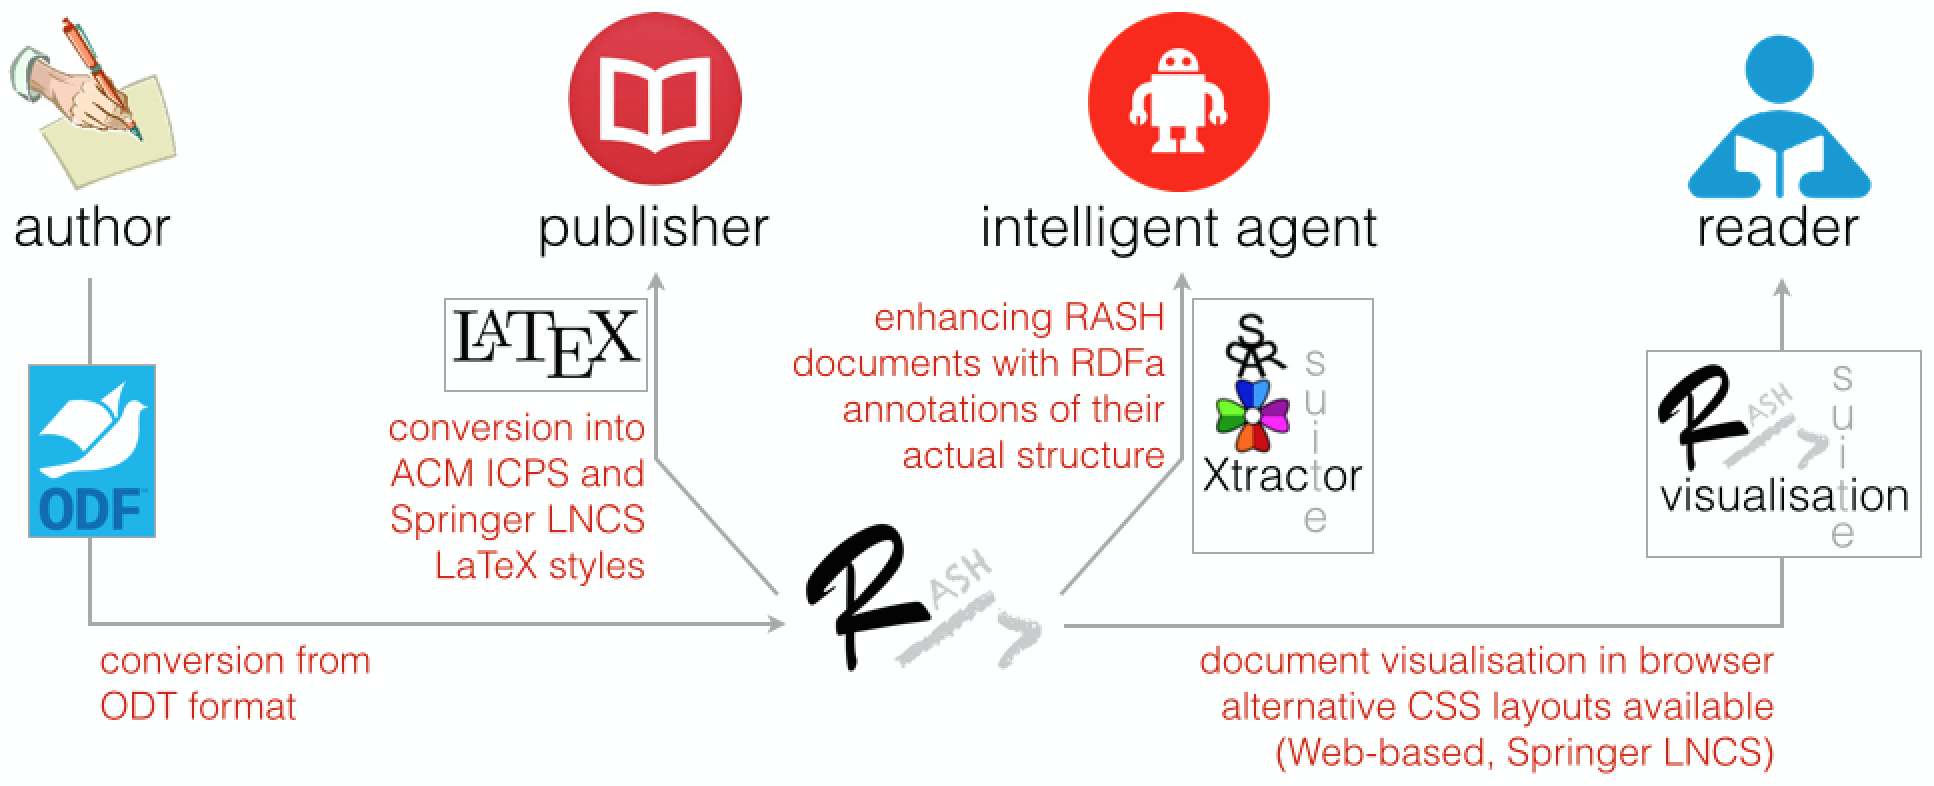
\includegraphics[width=\maxwidth{\textwidth}]{img/rash-demo-iswc2015-framework.png}
\caption{The RASH Framework and its components addressing needs of different users.}
\label{fig_framework}
\end{figure}


\section{Tools in the Framework}\label{sec_tools}

In this section we introduce all the tools shown in Fig.~\ref{fig_framework} that we have developed in order to support users in adopting RASH - all the tools are distributed under an ISC License or a CC-BY 4.0 International License.

{\bf Validation.} All the markup items in RASH are defined as a RelaxNG grammar and are compatible with HTML5. We have developed a script to enable RASH users to check their documents simultaneously both against the specific requirements in the RelaxNG grammar and also against the full set of HTML checks that the W3C Nu HTML Checker does for all HTML documents.

{\bf Visualisation.} The visualisation of RASH documents is rendered by the browser in the current form by means of appropriate CSS3 stylesheets and javascript scripts developed for this purpose. We are actually using some external libraries, i.e., Bootstrap and JQuery, in order to guarantee the current clear visualisation and for adding additional tools to the user. As an example, the RASH version of this paper is available at \url{https://rawgit.com/essepuntato/rash/master/papers/rash-demo-iswc2015.html}.

{\bf Conversion}. We have spent some efforts in preparing XSLT 2.0 documents for converting RASH documents into different LaTeX styles, such as ACM ICPS and Springer LNCS. This is, actually, one of the crucial steps to guarantee the use of RASH within international events\footnote{\url{https://github.com/essepuntato/rash/\#venues-that-have-adopted-rash-as-submission-format}} and to be able to publish RASH documents in the official LaTeX format as required by the organisation committee of such events. In addition, we have already developed another XSLT 2.0 document to perform conversions from OpenOffice documents into RASH documents, which allows authors to write a paper through the OpenOffice editor and then converting the related ODT file into RASH automatically.

{\bf Enhancement.} A recent development of the RASH Framework has concerned the automatic enrichment of RASH documents with RDFa annotations defining the actual structure of such documents in terms of the Document Component Ontology (DoCO) \cite{doco}. In particular, a Java application called {\em SPAR Xtractor suite} has been developed: it takes a RASH document as input and returns a new RASH document where all its markup elements have been annotated with their actual (structural) semantics.

\section{Conclusions}\label{sec_conclusions}

In this paper we have introduced the {\em RASH Framework}, i.e., a set of specifications and tools for writing academic articles in {\em RASH}. We have discussed the rationale behind the development of RASH, and we have presented the language with all the validation/visualisation/conversion/extraction tools we have developed so far. As immediate future developments, we plan to create additional scripts for extracting RDF statements from RASH documents according to SPAR Ontologies (\url{http://www.sparontologies.net}), and to develop additional XSLT documents in order to convert DOCX documents into RASH and to convert RASH documents into several formats for scholarly communications, such as EPUB, DocBook, and LaTeX IEEE styles.

\begin{thebibliography}{4}

\bibitem{force11} Bourne, P. E., Clark, T., Dale, R., de Waard, A., Herman, I., Hovy, E. H., \& Shotton, D. (2011). FORCE11 White Paper: Improving The Future of Research Communications and e-Scholarship. White paper, 28 October 2011. FORCE11. \url{https://www.force11.org/white\_paper}
\bibitem{linked-research} Capadisli, S., Riedl, R., \& Auer, S. (2015). Enabling Accessible Knowledge. In Proc. of CeDEM 2015. OA version available at \url{http://csarven.ca/enabling-accessible-knowledge}
\bibitem{doco} Constantin, A., Peroni, S., Pettifer, S., Shotton, D., \& Vitali, F. (in press). The Document Component Ontology (DoCO). To appear in Semantic Web. OA version available at \url{http://www.semantic-web-journal.net/system/files/swj1016.pdf}
\bibitem{patterns} Di Iorio, A., Peroni, S., Poggi, F., \& Vitali, F. (2014). Dealing with structural patterns of XML documents. Journal of the American Society for Information Science and Technology, 65(9): 1884--1900. \url{http://dx.doi.org/10.1002/asi.23088}
\bibitem{scholmd} Lin, T. T. Y., \& Beales, G. (2015). ScholarlyMarkdown Syntax Guide. Guide, 31 January 2015. \url{http://scholarlymarkdown.com/Scholarly-Markdown-Guide.html}
\bibitem{shotton-sempub} Shotton, D., Portwin, K., Klyne, G., \& Miles, A. (2009). Adventures in Semantic Publishing: Exemplar Semantic Enhancements of a Research Article. PLoS Computational Biology, 5(4): e1000361. \url{http://dx.doi.org/10.1371/journal.pcbi.1000361}

\end{thebibliography}

\end{document}